\documentclass[aspectratio=169,10pt]{beamer}
\hfuzz=12pt
\vfuzz=14pt

\usetheme{metropolis}
\metroset{block=fill, sectionpage=progressbar, numbering=fraction}

\usepackage{amsmath,amssymb}
\usepackage{tikz}
\usetikzlibrary{arrows.meta,positioning,calc}
\usepackage{array,booktabs}
\usepackage{xcolor}

\definecolor{giublue}{RGB}{30,58,138}
\definecolor{giuaccent}{RGB}{13,148,136}
\setbeamercolor{frametitle}{bg=giublue}
\setbeamercolor{progress bar}{fg=giuaccent}
\setbeamercolor{alerted text}{fg=giuaccent}
\setbeamerfont{title}{size=\large}
\setbeamerfont{subtitle}{size=\scriptsize}
\setbeamerfont{institute}{size=\scriptsize}
\setbeamerfont{date}{size=\tiny}

\title{Reinforcement Learning for Simple Adaptive Robot Behavior}
\subtitle{Literature review and project proposal}
\author{Nour Gaser \and Eman Saleh}
\institute{German International University}
\date{\today}

\newcommand{\E}{\mathbb{E}}
\newcommand{\refnum}[1]{{\footnotesize\color{giuaccent}[#1]}}

\hypersetup{pdftitle={Reinforcement Learning for Simple Adaptive Robot Behavior}, pdfauthor={Nour Gaser and Eman Saleh}}
\pdfstringdefDisableCommands{\def\translate#1{#1}}

\begin{document}

\maketitle

\begin{frame}{Roadmap}
  \tableofcontents
\end{frame}

% ============================================================
\section{Background}
% ============================================================

\begin{frame}{Social robots and adaptive behavior}
  {\footnotesize\itshape First, a brief shared vocabulary for the papers ahead --- for anyone less familiar with these ideas.}
  \vspace{0.4em}
  \begin{columns}[T]
    \begin{column}{0.5\textwidth}
      \textbf{Robot:} an embodied machine that senses, computes, and acts.

      \medskip
      \textbf{Social robot:} interacts with people using human-like cues and social rules.

      \medskip
      \textbf{Human--Robot Interaction:} the field --- robotics, AI, psychology, design --- studying how people and robots interact.
    \end{column}
    \begin{column}{0.46\textwidth}
      \textbf{Core challenges}
      \begin{itemize}\footnotesize
        \item Embodiment --- the body shapes interaction
        \item Autonomy --- how much the robot decides
        \item Trust --- whether people rely on it
      \end{itemize}
      \medskip
      \textbf{Signals we can use}
      \begin{itemize}\footnotesize
        \item Speech, gesture, gaze, proxemics (space)
        \item Gaze, repositioning, touch --- usable as a \emph{reward}
      \end{itemize}
    \end{column}
  \end{columns}
  \vspace{0.4em}
  \begin{block}{The idea in one sentence}
    A robot can learn online, from a person's social signals as a reward, to adapt simple social behaviors --- formalized as a Markov Decision Process and solved with lightweight RL.
  \end{block}
\end{frame}

\begin{frame}{Three ways a machine can learn}
  \begin{columns}[T]
    \begin{column}{0.33\textwidth}
      \textbf{Supervised}
      \begin{itemize}\footnotesize
        \item Learn input $\to$ correct label from examples.
        \item Needs large pre-labeled data; trained offline.
        \item E.g.\ an emotion classifier from labeled images.
      \end{itemize}
    \end{column}
    \begin{column}{0.33\textwidth}
      \textbf{Unsupervised}
      \begin{itemize}\footnotesize
        \item Find structure in unlabeled data.
        \item Clustering, dimensionality reduction.
        \item E.g.\ group users by interaction style.
      \end{itemize}
    \end{column}
    \begin{column}{0.33\textwidth}
      \textbf{Reinforcement}
      \begin{itemize}\footnotesize
        \item Learn by trial and error from a reward.
        \item No labels; adapts online.
        \item E.g.\ adjust distance if the person leans in or backs away.
      \end{itemize}
    \end{column}
  \end{columns}
  \vspace{0.8em}
  \begin{alertblock}{Why reinforcement learning here}
    The ``correct'' social behavior is person-specific, unknown in advance, and shifts during interaction. Supervised learning needs a labeled answer up front and cannot adapt mid-interaction. RL learns the answer from the interaction itself.
  \end{alertblock}
\end{frame}

\begin{frame}{The reinforcement-learning loop}
  \begin{columns}[c,onlytextwidth]
    \begin{column}{0.42\textwidth}
      \centering
      \resizebox{\linewidth}{!}{%
      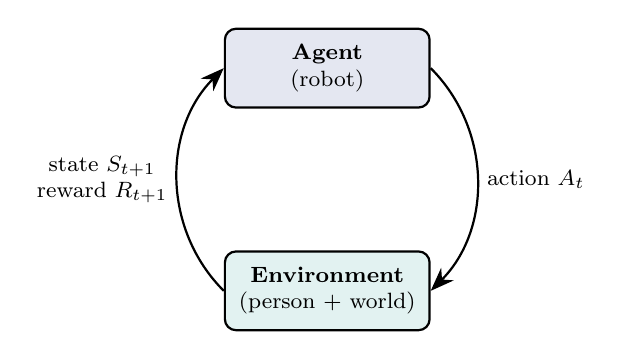
\begin{tikzpicture}[
        node distance=1.4cm,
        box/.style={draw, rounded corners, minimum width=2.6cm, minimum height=1cm, align=center, thick},
        every node/.style={font=\footnotesize}]
        \node[box, fill=giublue!12] (agent) {\textbf{Agent}\\(robot)};
        \node[box, fill=giuaccent!12, below=1.8cm of agent] (env) {\textbf{Environment}\\(person + world)};
        \draw[-{Stealth[length=3mm]}, thick]
          (agent.east) to[bend left=45] node[right, midway]{action $A_t$} (env.east);
        \draw[-{Stealth[length=3mm]}, thick]
          (env.west) to[bend left=45] node[left, midway, align=center]{state $S_{t+1}$\\reward $R_{t+1}$} (agent.west);
      \end{tikzpicture}%
      }
    \end{column}
    \begin{column}{0.50\textwidth}
      At each step $t$ the agent:
      \begin{enumerate}\footnotesize
        \item observes state $S_t$,
        \item takes action $A_t$ via policy $\pi(a\mid s)$,
        \item receives reward $R_{t+1}$,
        \item lands in state $S_{t+1}$.
      \end{enumerate}
      \medskip
      \textbf{Goal:} find $\pi$ maximizing the expected discounted return
      \[
        G_t=\textstyle\sum_{k\ge 0}\gamma^{k}R_{t+k+1},\quad \gamma\in[0,1).
      \]
      \textbf{Value} $Q(s,a)$ = expected return from taking $a$ in $s$.
    \end{column}
  \end{columns}
  \vfill
  {\footnotesize\raggedright Formalized as a Markov Decision Process $\langle S,A,P,R,\gamma\rangle$: the next state depends only on the current $(s,a)$. \refnum{Sutton2018}\par}
\end{frame}

\begin{frame}{Q-learning}
  \textbf{Idea:} learn the value of each (state, action) pair directly --- no model of the world needed.
  \vspace{0.4em}
  \begin{block}{Q-learning update (Watkins \& Dayan, 1992)}
    \[
      Q(s,a)\;\leftarrow\;Q(s,a)\;+\;\alpha\Big[\,\underbrace{r+\gamma\max_{a'}Q(s',a')}_{\text{target}}\;-\;Q(s,a)\,\Big]
    \]
    \footnotesize $\alpha$: learning rate \quad $\gamma$: discount \quad $r$: observed reward
  \end{block}
  \vspace{0.2em}
  \begin{columns}[T]
    \begin{column}{0.5\textwidth}
      \textbf{Exploration vs.\ exploitation}
      \begin{itemize}\footnotesize
        \item Must try new actions and use known-good ones.
        \item $\varepsilon$-greedy: random action with probability $\varepsilon$, else $\arg\max_a Q(s,a)$; decay $\varepsilon$ over time.
      \end{itemize}
    \end{column}
    \begin{column}{0.5\textwidth}
      \textbf{Tabular vs.\ approximation}
      \begin{itemize}\footnotesize
        \item Tabular: one value per $(s,a)$ --- good for small, discrete spaces.
        \item Large or continuous spaces $\to$ function approximation (Deep Q-Networks).
      \end{itemize}
    \end{column}
  \end{columns}
\end{frame}

\begin{frame}{Policy gradients and human feedback}
  \begin{columns}[T]
    \begin{column}{0.5\textwidth}
      \textbf{Policy gradients (REINFORCE)}
      \begin{itemize}\footnotesize
        \item Directly tune a parameterized policy $\pi_\theta$ toward higher reward.
        \item Suited to continuous actions: distance, speed, timing.
        \item Used by Mitsunaga et al.\ to adapt proxemics, gaze, and timing on a social robot. \refnum{Mitsunaga2005}
      \end{itemize}
    \end{column}
    \begin{column}{0.5\textwidth}
      \textbf{Interactive RL (human feedback)}
      \begin{itemize}\footnotesize
        \item The human supplies the reward signal.
        \item TAMER: non-experts shape an agent via approval / disapproval. \refnum{Knox2009}
        \item Cuts the number of trials needed --- important on hardware.
      \end{itemize}
    \end{column}
  \end{columns}
  \vspace{0.6em}
  \begin{alertblock}{The hardware reality}
    Every real trial costs time, battery, and joint wear. Sample efficiency matters, and policies that work in simulation can fail on the physical robot --- the ``reality gap''.
  \end{alertblock}
\end{frame}

\begin{frame}{Learning from demonstration}
  \begin{columns}[T]
    \begin{column}{0.55\textwidth}
      \textbf{Teach by showing}, not by coding or rewarding. \refnum{Argall2009}
      \begin{itemize}
        \item Intuitive for non-experts --- people teach by demonstrating.
        \item Kinesthetic teaching: set joint stiffness to zero, physically move the robot's limb, record the trajectory, replay it.
      \end{itemize}
    \end{column}
    \begin{column}{0.43\textwidth}
      \begin{block}{Pairing it with RL}
        A demonstration gives a good starting policy; RL then refines it through interaction --- easing RL's slow cold-start.
      \end{block}
    \end{column}
  \end{columns}
\end{frame}

\begin{frame}{Personalization in long-term HRI}
  \begin{columns}[T]
    \begin{column}{0.56\textwidth}
      \textbf{Why adapt at all?}
      \begin{itemize}\footnotesize
        \item Short interactions hide the hard part: sustaining engagement over many sessions. \refnum{Irfan2019}
        \item Adaptation counters the novelty effect --- interest fades once a robot stops being new.
        \item Built on user modeling and incremental learning. \refnum{Irfan2021}
      \end{itemize}
    \end{column}
    \begin{column}{0.42\textwidth}
      \textbf{Static vs.\ dynamic}
      \begin{itemize}\footnotesize
        \item Static: fix a profile once (a questionnaire).
        \item Dynamic: adjust in real time to live social signals.
      \end{itemize}
    \end{column}
  \end{columns}
  \vspace{0.6em}
  \begin{alertblock}{The ethical edge \refnum{Pollmann2023}}
    The same personalization that improves user experience can be used to steer a person against their own autonomy. Adaptive systems need explicit ethical guardrails.
  \end{alertblock}
\end{frame}

\begin{frame}{A recurring pattern: games and simulation}
  As we read across this field, two patterns showed up again and again --- worth naming before the papers:
  \begin{itemize}
    \item \textbf{Games as metaphor and as tooling.} Game engines and ``serious games'' recur everywhere --- Unity (Gonzalez), \emph{Assistive Gym} (Wang), a cooking game (Zedda), a storytelling activity (Tozadore).
    \item \textbf{It cuts across robot types.} The same toolkit serves social humanoids (NAO, Pepper) \emph{and} industrial cobots (the UR3e arm) alike.
    \item \textbf{Simulation is nearly unavoidable} --- it is safe, cheap, and fast for the many trials RL needs.
  \end{itemize}
  \vspace{0.2em}
  \begin{alertblock}{The catch}
    Training in simulation always introduces the \emph{reality gap} (sim-to-real): a policy that works in a clean simulator can fail on a noisy physical robot. Every one of these papers has to confront it --- and so will we.
  \end{alertblock}
\end{frame}

% ============================================================
\section{Why these papers}
% ============================================================

\begin{frame}{Why these papers}
  {\footnotesize What we explore: \emph{can a robot learn, online, to adapt simple social behaviors from a person's signals --- and how is this being done now?}}
  \vspace{0.5em}
  \begin{columns}[T]
    \begin{column}{0.46\textwidth}
      \textbf{Foundational references} (some older)
      \begin{itemize}\footnotesize
        \item Used to build the vocabulary in the previous slides: RL, learning from demonstration, personalization, ethics.
        \item Deliberately allowed to be older --- core definitions and methods do not expire.
      \end{itemize}
    \end{column}
    \begin{column}{0.5\textwidth}
      \textbf{Four modern papers we analyze in depth}
      \begin{itemize}\footnotesize
        \item Tozadore (2018): adaptation on a humanoid (NAO), rule-based --- the pre-RL baseline.
        \item Gonzalez-Santocildes (2024): RL learns comfort-based adaptation.
        \item Zedda (2023$\to$2025): RL for engagement on a humanoid, simulation \emph{then} a real 28-user study --- closest task match.
        \item Wang (2025): preference-based RL --- the current frontier.
      \end{itemize}
    \end{column}
  \end{columns}
  \vspace{0.4em}
  \begin{block}{Why this set}
    Together they trace the field's trajectory --- rule-based $\to$ RL $\to$ preference-based; hand-designed $\to$ learned reward; simulation $\to$ real study --- and let us locate where our own project sits.
  \end{block}
\end{frame}

% ============================================================
\section{Paper 1: Gonzalez-Santocildes et al.\ (2024)}
% ============================================================

\begin{frame}{Problem and setup}
  \footnotesize \emph{Adaptive Robot Behavior Based on Human Comfort Using Reinforcement Learning}, IEEE Access. \refnum{Gonzalez2024}
  \vspace{0.4em}
  \begin{columns}[T]
    \begin{column}{0.52\textwidth}
      \textbf{The problem}
      \begin{itemize}\footnotesize
        \item Most RL for robotics ignores the human --- it optimizes task success, not comfort.
        \item Prior comfort work is largely theoretical and not replicable.
      \end{itemize}
      \textbf{Contribution}
      \begin{itemize}\footnotesize
        \item An open-source, parametric Unity environment the community can reuse.
        \item A comfort reward function whose strictness is set by one parameter.
      \end{itemize}
    \end{column}
    \begin{column}{0.46\textwidth}
      \textbf{Setup (worth noting)}
      \begin{itemize}\footnotesize
        \item Robot: UR3e --- an industrial arm, not a social humanoid.
        \item Task: pick-and-place near a moving simulated human.
        \item Comfort here is physical (distance, speed), not social.
        \item Algorithm: SAC (deep RL for continuous control).
      \end{itemize}
    \end{column}
  \end{columns}
\end{frame}

\begin{frame}{Methodology}
  \footnotesize
  Standard task reward, minus a comfort penalty the user can switch on and weight:
  \[
    R = k_1 F_{\text{task1}} + k_2 F_{\text{task2}} + k_3 F_{\text{task3}} \;-\; F_{\text{comfort}}(C_l, N_c)
  \]
  \[
    F_{\text{comfort}}(C_l,N_c) = \alpha\, F_{\text{conf1}}(C_l,N_c)\;+\;\beta\, F_{\text{conf2}}(C_l,N_c)
  \]
  \begin{columns}[T]
    \begin{column}{0.5\textwidth}
      \begin{itemize}\footnotesize
        \item $F_{\text{conf1}}$: penalty on distance (too close hurts reward).
        \item $F_{\text{conf2}}$: penalty on joint speed (too fast hurts reward).
        \item $\alpha,\beta$: weights; set both to $0$ and it is plain task RL.
      \end{itemize}
    \end{column}
    \begin{column}{0.5\textwidth}
      \textbf{Why ``comfort levels'' ($C_l$ of $N_c$)?}
      \begin{itemize}\footnotesize
        \item Comfort is discretized (10 levels), each trained separately --- easier than one policy over a continuum.
        \item The level sets where the penalty threshold sits.
        \item Static per run = controlled variation: change one thing, attribute the effect cleanly.
      \end{itemize}
    \end{column}
  \end{columns}
\end{frame}

\begin{frame}{Results}
  \begin{center}
    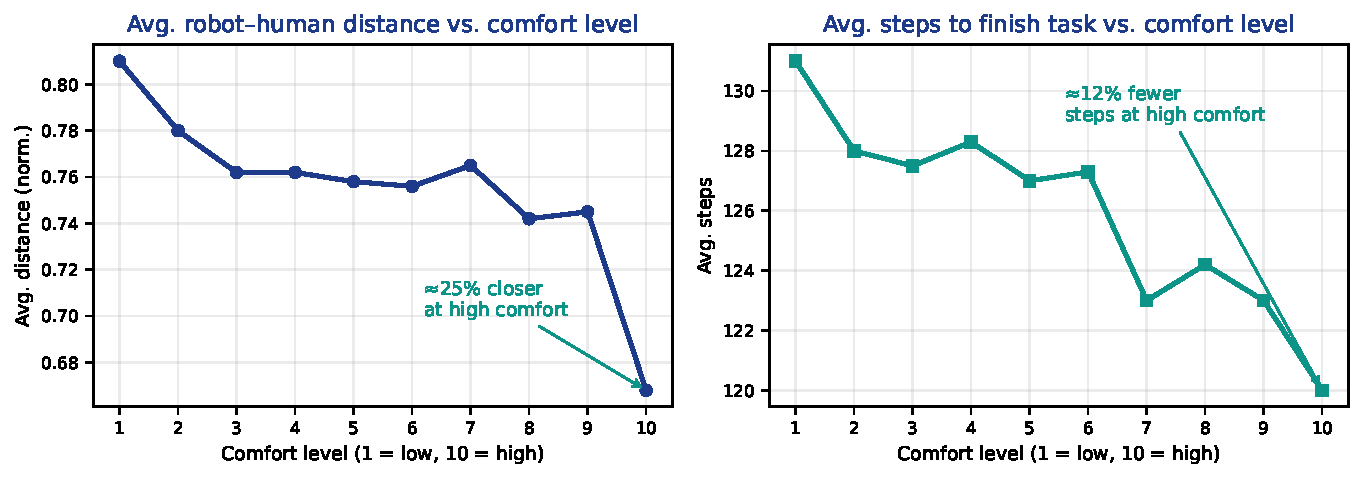
\includegraphics[width=0.92\linewidth]{gonzalez_results.pdf}
  \end{center}
  \vspace{-0.3em}
  {\footnotesize As comfort rises, the robot works closer ($\approx$25\% less distance) and faster ($\approx$12\% fewer steps). Trained with SAC (30M steps, $\approx$4.4 days on a GPU). \emph{Charts redrawn from Gonzalez et al.\ (2024), Figs.\ 5--6; values approximate.} \refnum{Gonzalez2024}}
\end{frame}

\begin{frame}{Critique and relevance}
  \begin{columns}[T]
    \begin{column}{0.5\textwidth}
      \textbf{Strengths}
      \begin{itemize}\footnotesize
        \item Clean controlled result: behavior tracks the comfort parameter.
        \item Open, replicable environment.
      \end{itemize}
      \textbf{Gaps}
      \begin{itemize}\footnotesize
        \item Comfort is set manually; measuring it live from a person is unsolved (they suggest HR/EEG/a button).
        \item Only move-pick-place tasks.
        \item Physical/industrial comfort, not social; not a humanoid.
        \item Validated only in simulation.
      \end{itemize}
    \end{column}
    \begin{column}{0.5\textwidth}
      \textbf{Relevance to us}
      \begin{itemize}\footnotesize
        \item We borrow the proven idea --- comfort in the reward --- and add the missing piece: a live comfort signal from a robot's own sensors.
        \item We move from physical toward social comfort.
        \item A small discrete state space lets us use tabular Q-learning rather than SAC: lighter and laptop-trainable.
      \end{itemize}
    \end{column}
  \end{columns}
\end{frame}

% ============================================================
\section{Paper 2: Zedda et al.\ (2023\,$\to$\,2025)}
% ============================================================
 
\begin{frame}{Problem and setup}
  \footnotesize \emph{An Adaptive Behaviour-Based Strategy for SARs interacting with Older Adults with MCI\ldots}, SARs workshop @ CHI 2023 \refnum{Zedda2023} --- extended as \emph{Adaptive Humanoid Robot Behaviour\ldots through Reinforcement Learning}, \emph{Behaviour \& Information Technology}, 2025. \refnum{Zedda2025}
  \vspace{0.4em}
  \begin{columns}[T]
    \begin{column}{0.52\textwidth}
      \textbf{The problem}
      \begin{itemize}\footnotesize
        \item Cognitive training for older adults with MCI is repetitive --- leading to disengagement and dropout.
        \item A socially assistive robot can help --- \emph{if} it adapts its behavior to the user's state.
      \end{itemize}
      \textbf{Contribution}
      \begin{itemize}\footnotesize
        \item A Q-learning strategy that picks verbal and non-verbal actions to keep engagement high.
        \item Two selectable robot personalities (extravert / introvert).
      \end{itemize}
    \end{column}
    \begin{column}{0.46\textwidth}
      \textbf{We follow one team across two papers}
      \begin{itemize}\footnotesize
        \item \textbf{2023 (workshop):} the method, validated in \emph{simulation only} --- real study deferred.
        \item \textbf{2025 (journal):} same method, now run as a real \textbf{28-user} study --- the gap the workshop left open.
        \item Robot: Pepper --- NAO's sibling (same maker, same NAOqi SDK), so methods transfer.
        \item Task: a ``cooking'' serious game (8 questions in 2023, 16 in 2025).
      \end{itemize}
    \end{column}
  \end{columns}
\end{frame}
 
\begin{frame}{Methodology --- the RL model}
  \footnotesize Tabular Q-learning, $Q(s,a)$ table, $\varepsilon$-greedy; model-free, off-policy. State $=$ engagement $\times$ answer $\Rightarrow$ 6 states; 3 actions.
  \vspace{0.3em}
  \begin{columns}[T]
    \begin{column}{0.34\textwidth}
      \textbf{State} (6)
      \begin{itemize}\footnotesize
        \item Engagement L / I / H, derived from gaze $+$ smile
        \item Answer right / wrong
        \item $\Rightarrow$ six (engagement, answer) states
      \end{itemize}
    \end{column}
    \begin{column}{0.30\textwidth}
      \textbf{Actions (3)}
      \begin{itemize}\footnotesize
        \item engaging / dynamic
        \item neutral
        \item stimulating (re-engage)
      \end{itemize}
      {\scriptsize each filtered through personality: pitch, rate, volume, gesture}
    \end{column}
    \begin{column}{0.34\textwidth}
      \textbf{Reward} $R(s,a)$
      \begin{itemize}\footnotesize
        \item Engagement: $H{=}{+}10$, $I{=}{-}2.5$, $L{=}{-}5$
        \item Answer: right ${+}10$, wrong ${-}5$
        \item weighted by user-profile probabilities; ${-}0.05t$ per step
      \end{itemize}
    \end{column}
  \end{columns}
  \vspace{0.3em}
  \begin{alertblock}{A detail we tracked across both versions}
    The discount rose from $\gamma=0.05$ (2023) to $\gamma=0.2$ (2025) --- still myopic (the agent mostly values the \emph{immediate} engagement response, close to a contextual bandit), but less extreme. Learning rate stays high at $\alpha=0.8$; $\varepsilon$ decays from $1$ to $0.2$.
  \end{alertblock}
\end{frame}
 
\begin{frame}{Results --- simulation (the convergence check)}
  \begin{columns}[c,onlytextwidth]
    \begin{column}{0.52\textwidth}
      \centering
      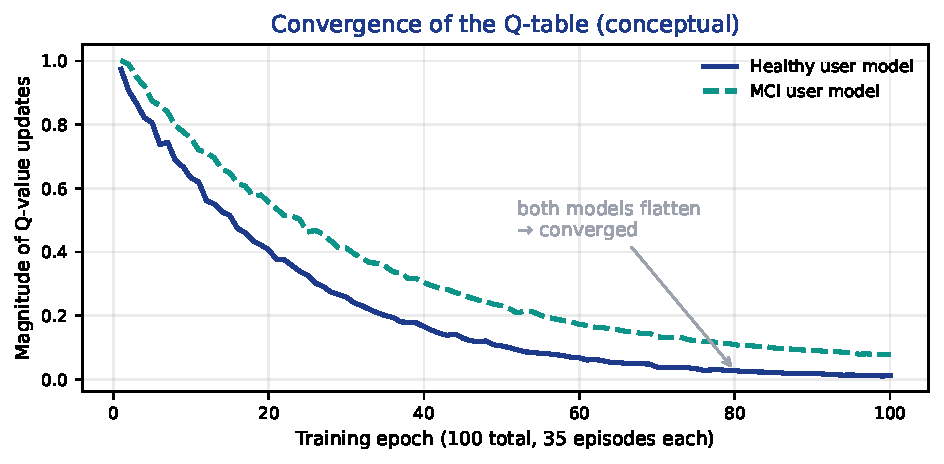
\includegraphics[width=\linewidth]{zedda_convergence.pdf}
    \end{column}
    \begin{column}{0.46\textwidth}
      \footnotesize
      \textbf{Training}: Python; 100 simulated users $\times$ 35 iterations; two user models (healthy, MCI) plus ``optimal'' and ``inactive'' probe profiles.
      \medskip
      \textbf{Outcome}
      \begin{itemize}\footnotesize
        \item Converges within $\sim$15 iterations; the QL policy beats the random policy for \emph{every} profile.
        \item MCI plateaus below healthy --- expected, as MCI users disengage more easily.
        \item Learned Q-table: MCI users need more \emph{stimulating} actions, healthy users more \emph{engaging} ones.
      \end{itemize}
    \end{column}
  \end{columns}
  \vspace{0.2em}
  {\scriptsize Curves redrawn from Zedda et al.\ (2025), Fig.\ 3 (four user profiles; QL solid vs.\ random dashed). \refnum{Zedda2025}}
\end{frame}
 
\begin{frame}{Results --- the real 28-user study (new in 2025)}
  \footnotesize Within-subjects: each of 28 users (age 20--72) met both an \textbf{adaptive} robot (trained Q-table) and a \textbf{random} robot; order and personality counterbalanced; ethics-approved.
  \vspace{0.3em}
  \begin{columns}[T]
    \begin{column}{0.33\textwidth}
      \textbf{RQ1 --- can users tell?}
      \begin{itemize}\footnotesize
        \item Yes. Adaptive rated more adaptive in animations ($p{\approx}0.0001$) and verbal feedback ($p{\approx}0.0005$).
      \end{itemize}
    \end{column}
    \begin{column}{0.33\textwidth}
      \textbf{RQ2 --- engagement / UX}
      \begin{itemize}\footnotesize
        \item \textbf{86\%} preferred the adaptive robot.
        \item Higher engagement (UES) and enjoyment ($4.57$ vs $3.96$).
        \item Comfort difference \emph{not} significant.
      \end{itemize}
    \end{column}
    \begin{column}{0.33\textwidth}
      \textbf{RQ3 --- perception (Godspeed)}
      \begin{itemize}\footnotesize
        \item Likeability $4.50$ vs $3.94$ *
        \item Anthropomorphism $3.6$ vs $2.90$ *
        \item Perceived intelligence $3.89$ vs $3.6$ (n.s.)
      \end{itemize}
    \end{column}
  \end{columns}
  \vspace{0.3em}
  \begin{block}{}
    \footnotesize Simulation showed the algorithm \emph{converges}; this study shows the interaction \emph{works} --- users notice, prefer, and warm to the adaptive robot. ($*$ significant, $p<0.05$.) \refnum{Zedda2025}
  \end{block}
\end{frame}
 
\begin{frame}{Critique and relevance}
  \begin{columns}[T]
    \begin{column}{0.5\textwidth}
      \textbf{Strengths}
      \begin{itemize}\footnotesize
        \item The closest match to our project: humanoid $+$ tabular Q-learning $+$ engagement reward --- now carried all the way to a \emph{real} study.
        \item Clean simulation-then-real pipeline; reusable instruments (within-subjects design, UES, Godspeed).
      \end{itemize}
      \textbf{Gaps}
      \begin{itemize}\footnotesize
        \item Reward weights still hand-set from prior qualitative work (their own stated future work).
        \item Only 3 actions; personality fixed per session; low $\gamma$ limits long-horizon credit.
        \item Single short session, $N{=}28$, lab setting, no formal cognitive assessment.
      \end{itemize}
    \end{column}
    \begin{column}{0.5\textwidth}
      \textbf{Relevance to us}
      \begin{itemize}\footnotesize
        \item Validates our method \emph{end-to-end}: tabular Q-learning for engagement on a humanoid works with real users, not just in simulation.
        \item Pepper and NAO share the NAOqi SDK, so their state and actions map across.
        \item Gives us a proven study template: adaptive vs.\ random, within-subjects, with UES $+$ Godspeed.
      \end{itemize}
    \end{column}
  \end{columns}
\end{frame}


% ============================================================
\section{Paper 3: Wang et al.\ (2025)}
% ============================================================
\begin{frame}{Personalization in Human-Robot Interaction through
Preference-based Action Representation Learning}

\footnotesize
\textbf{Robots in Today’s World}

\begin{itemize}\footnotesize
    \item Robots are widely used:
    \begin{itemize}
        \item Delivery
        \item Assistance
        \item Companionship
    \end{itemize}
    \item Machine learning improves robot intelligence
    \item But human interaction remains challenging
\end{itemize}
\end{frame}

% -------------------- Slide 3 --------------------
\begin{frame}{Industrial vs Human-Robot Systems}
\footnotesize
\begin{columns}[T]
\begin{column}{0.5\textwidth}
\textbf{Industrial Robots}
\begin{itemize}\footnotesize
    \item Fixed tasks
    \item Controlled environments
    \item Repetitive behavior
\end{itemize}
\end{column}

\begin{column}{0.5\textwidth}
\textbf{Human-Interactive Robots}
\begin{itemize}\footnotesize
    \item Dynamic environments
    \item Must adapt to users
    \item No single correct behavior
\end{itemize}
\end{column}
\end{columns}
\end{frame}

% -------------------- Slide 4 --------------------
\begin{frame}{Why Personalization Matters}
\footnotesize
\textbf{Same task, different users}

\begin{itemize}\footnotesize
    \item Feeding a baby → fast movement
    \item Feeding an elderly person → slow and careful
\end{itemize}

\vspace{0.5em}
\textbf{Key insight:} One behavior does not fit all users
\end{frame}

% -------------------- Slide 5 --------------------
\begin{frame}{Rule-Based Methods}
\footnotesize
\textbf{Early approach}

\begin{itemize}\footnotesize
    \item Hand-crafted rules
    \item Example: spoon → mouth movement
    \item Food → pick and serve
\end{itemize}

\vspace{0.5em}
\textbf{Limitations}
\begin{itemize}\footnotesize
    \item Cannot cover all situations
    \item Complex real-world interactions
    \item High design cost
\end{itemize}
\end{frame}

% -------------------- Slide 6 --------------------
\begin{frame}{Learning-Based Methods}
\footnotesize
\begin{itemize}\footnotesize
    \item Robots learn from experience
    \item Improve over time
    \item Based on Reinforcement Learning
\end{itemize}
\end{frame}

% -------------------- Slide 7 --------------------
\begin{frame}{Preference-Based Reinforcement Learning}
\footnotesize
\textbf{PbRL idea}

\begin{itemize}\footnotesize
    \item Show two behaviors to user
    \item User selects preferred one
    \item Robot learns preferences
\end{itemize}

\vspace{0.5em}
\textbf{Advantage:} No manual reward design

\vspace{0.5em}
\textbf{Problem:} Requires learning from scratch
\end{frame}

% -------------------- Slide 8 --------------------
\begin{frame}{Problem with Fine-Tuning}
\footnotesize
\textbf{Issue}

\begin{itemize}\footnotesize
    \item Pretrained robots already know tasks
\end{itemize}

\textbf{But fine-tuning causes:}
\begin{itemize}\footnotesize
    \item Loss of learned skills
    \item Performance degradation
\end{itemize}

\vspace{0.5em}
\textbf{Example:} Safe drinking becomes unstable after adaptation
\end{frame}

% -------------------- Slide 9 --------------------
\begin{frame}{Key Trade-off}
\footnotesize
\begin{itemize}\footnotesize
    \item Training from scratch → too much data
    \item Fine-tuning → damages performance
\end{itemize}

\vspace{0.5em}
\textbf{Need:} A better balance between both
\end{frame}

% -------------------- Slide 10 --------------------
\begin{frame}{PbARL Idea}
\footnotesize
\begin{columns}[T,onlytextwidth]
\begin{column}{0.42\textwidth}
\textbf{Core concept}

\begin{itemize}\footnotesize
    \item Keep pretrained policy fixed
    \item Add adaptation layer
\end{itemize}

\vspace{0.5em}
\textbf{Key idea:}
\begin{itemize}\footnotesize
    \item Learn action representations
    \item Adjust behavior via preferences
\end{itemize}

\textbf{Result:} Personalization without forgetting skills
\end{column}
\begin{column}{0.55\textwidth}
\centering
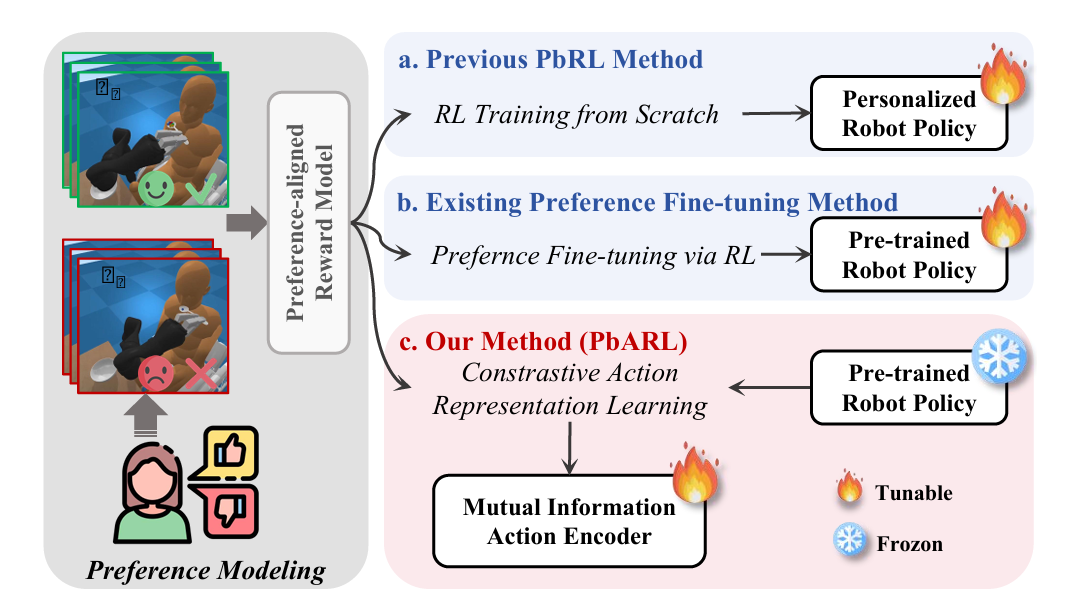
\includegraphics[width=\linewidth,height=0.72\textheight,keepaspectratio]{prism-uploads/Screenshot 2026-06-08 140211.png}
\end{column}
\end{columns}
\end{frame}

% -------------------- Slide 11 --------------------
\begin{frame}{Latent Action Space}
\footnotesize
\begin{columns}[T,onlytextwidth]
\begin{column}{0.40\textwidth}
\begin{itemize}\footnotesize
    \item Map actions into latent space
\end{itemize}

\textbf{Captures:}
\begin{itemize}\footnotesize
    \item Fast $\leftrightarrow$ slow
    \item Safe $\leftrightarrow$ risky
    \item Gentle $\leftrightarrow$ aggressive
\end{itemize}

\vspace{0.5em}
\textbf{Benefit:} Easier preference modeling
\end{column}
\begin{column}{0.57\textwidth}
\centering
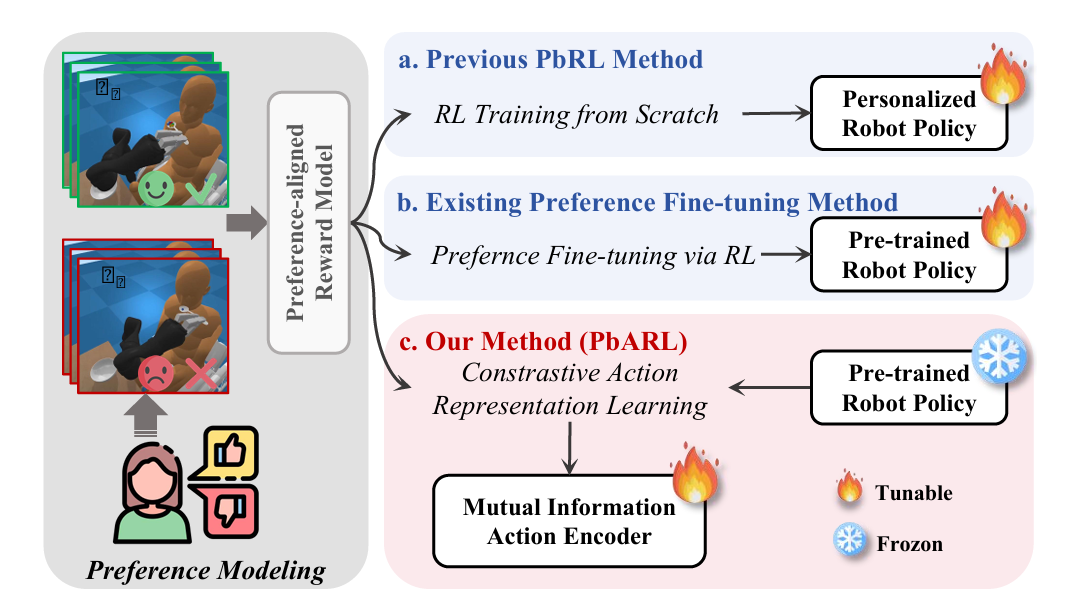
\includegraphics[width=\linewidth,height=0.72\textheight,keepaspectratio]{prism-uploads/Screenshot 2026-06-08 140211.png}
\end{column}
\end{columns}
\end{frame}

% -------------------- Slide 12 --------------------
\begin{frame}{PbARL Components}
\footnotesize
\begin{columns}[T,onlytextwidth]
\begin{column}{0.38\textwidth}
\begin{enumerate}\footnotesize
    \item Pretrained policy (task knowledge)
    \item Preference reward model
    \item Conditional VAE (cVAE)
\end{enumerate}
\end{column}
\begin{column}{0.59\textwidth}
\centering
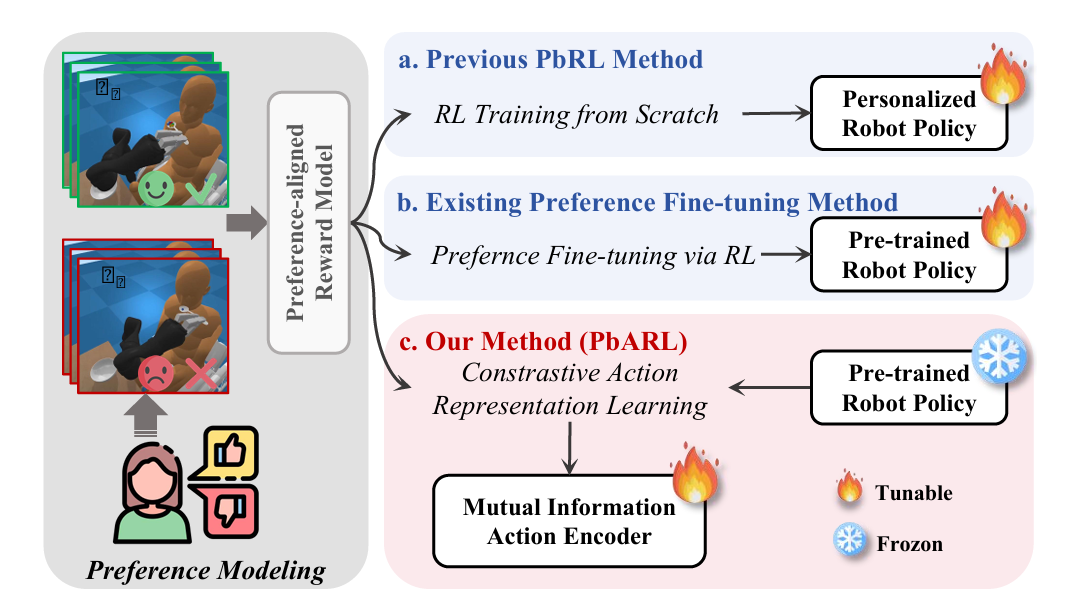
\includegraphics[width=\linewidth,height=0.72\textheight,keepaspectratio]{prism-uploads/Screenshot 2026-06-08 140211.png}
\end{column}
\end{columns}
\end{frame}

% -------------------- Slide 13 --------------------
\begin{frame}{Conditional VAE (cVAE)}
\footnotesize
\begin{columns}[T,onlytextwidth]
\begin{column}{0.42\textwidth}
\begin{itemize}\footnotesize
    \item Encoder: (state, action) $\to$ latent space
    \item Decoder: latent $\to$ reconstructed action
\end{itemize}

\vspace{0.5em}
\textbf{Meaning:}
\begin{itemize}\footnotesize
    \item Understand actions
    \item Reconstruct actions
\end{itemize}

\textbf{Benefit:} State-aware and realistic behavior
\end{column}
\begin{column}{0.55\textwidth}
\centering
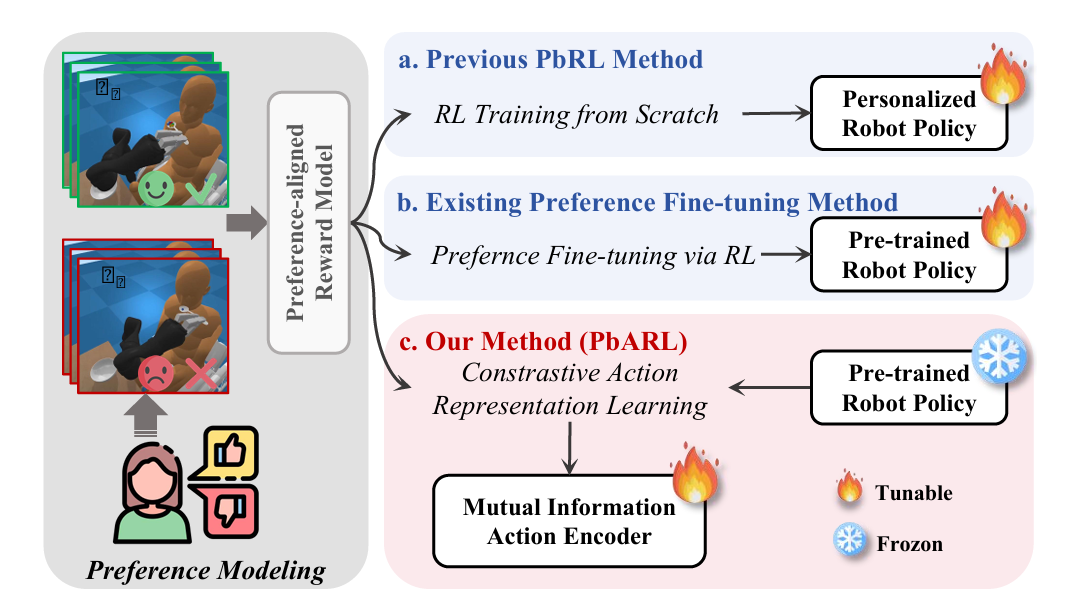
\includegraphics[width=\linewidth,height=0.72\textheight,keepaspectratio]{prism-uploads/Screenshot 2026-06-08 140211.png}
\end{column}
\end{columns}
\end{frame}

% -------------------- Slide 14 --------------------
\begin{frame}{Training Objectives}
\footnotesize
\begin{columns}[T,onlytextwidth]
\begin{column}{0.42\textwidth}
\begin{itemize}\footnotesize
    \item Reconstruction loss $\to$ preserve actions
    \item Preference loss $\to$ match user preferences
    \item KL loss $\to$ smooth latent space
    \item Dynamics loss $\to$ physical feasibility
\end{itemize}

\vspace{0.5em}
\textbf{Goal:} Safe and personalized behavior
\end{column}
\begin{column}{0.55\textwidth}
\centering
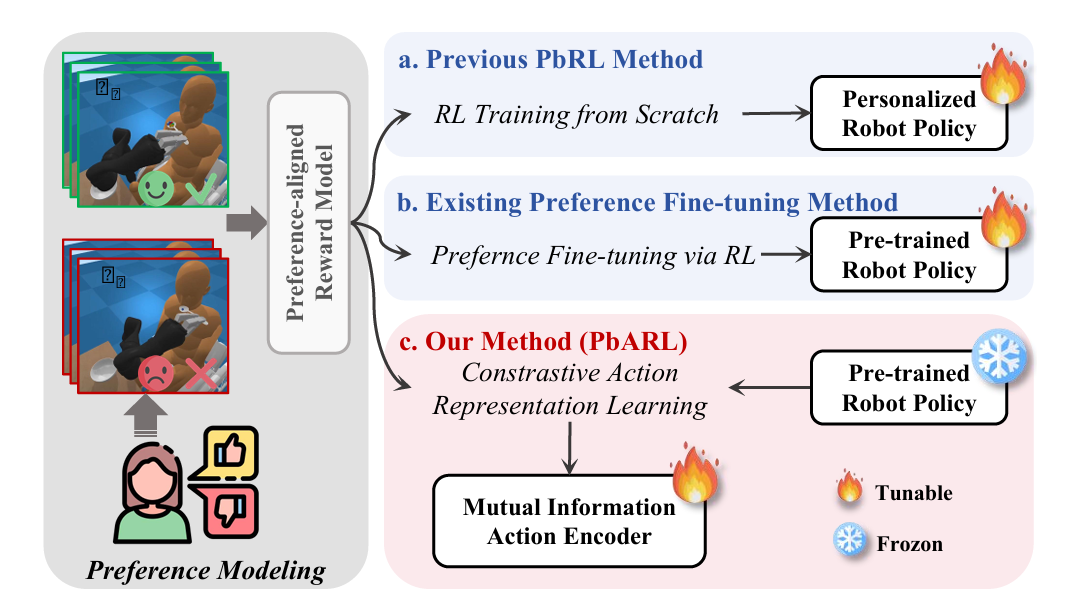
\includegraphics[width=\linewidth,height=0.72\textheight,keepaspectratio]{prism-uploads/Screenshot 2026-06-08 140211.png}
\end{column}
\end{columns}
\end{frame}

% -------------------- Slide 15 --------------------
\begin{frame}{PbARL Pipeline}
\footnotesize
\begin{columns}[T,onlytextwidth]
\begin{column}{0.38\textwidth}
\begin{itemize}\footnotesize
    \item Observe state
    \item Generate candidate actions
    \item Encode into latent space
    \item Evaluate preferences
    \item Re-rank actions
    \item Select best action
\end{itemize}
\end{column}
\begin{column}{0.59\textwidth}
\centering
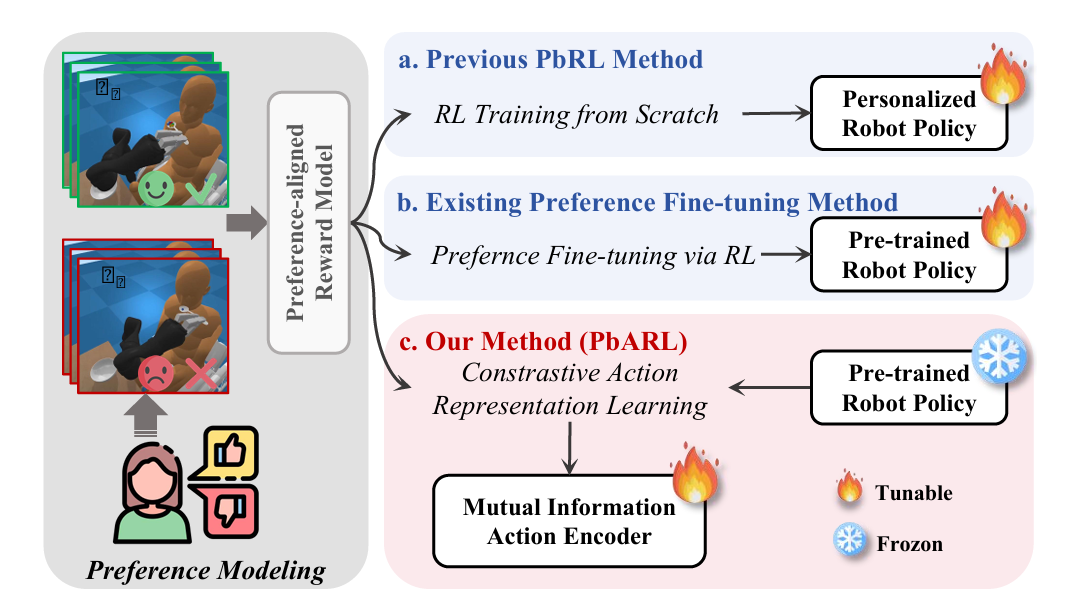
\includegraphics[width=\linewidth,height=0.72\textheight,keepaspectratio]{prism-uploads/Screenshot 2026-06-08 140211.png}
\end{column}
\end{columns}
\end{frame}

% -------------------- Slide 16 --------------------
\begin{frame}{Experiments Setup}
\footnotesize
\textbf{Tasks:}
\begin{itemize}\footnotesize
    \item Feeding
    \item Drinking
    \item Scratching
\end{itemize}

\textbf{Users:}
\begin{itemize}\footnotesize
    \item Neutral
    \item Cautious
    \item Impatient
\end{itemize}

\textbf{Methods:}
\begin{itemize}\footnotesize
    \item Pretrained policy
    \item PbRL-HRI
    \item Fine-tuning
    \item PbARL
\end{itemize}
\end{frame}

% -------------------- Slide 17 --------------------
\begin{frame}{Results}
\footnotesize
\begin{columns}[T,onlytextwidth]
\begin{column}{0.45\textwidth}
\begin{itemize}\footnotesize
    \item PbRL-HRI → needs many feedback samples
    \item Fine-tuning → reduces performance
    \item Pretrained → not personalized
    \item PbARL → best trade-off
\end{itemize}

\vspace{0.5em}
\textbf{Conclusion:} Best balance between performance and personalization
\end{column}
\begin{column}{0.52\textwidth}
\centering
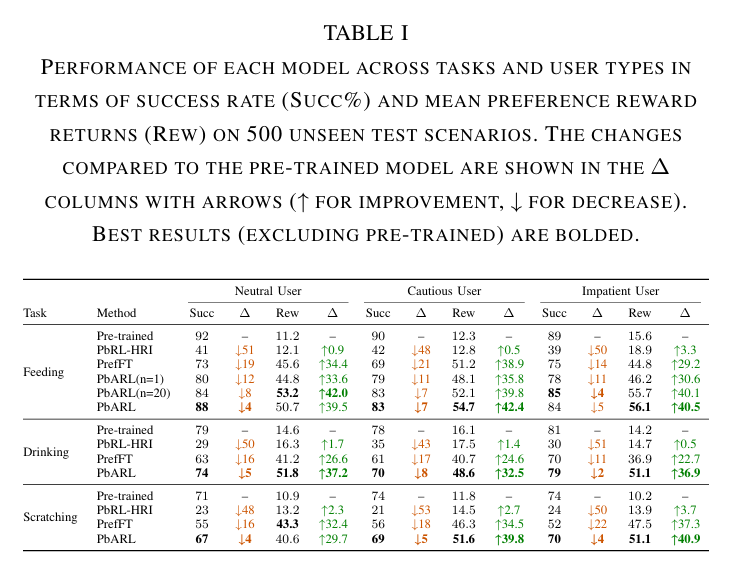
\includegraphics[width=\linewidth,height=0.72\textheight,keepaspectratio]{uploads/Screenshot 2026-06-08 140015.png}
\end{column}
\end{columns}
\end{frame}

% -------------------- Slide 18 --------------------
\begin{frame}{Ablation Study}
\footnotesize
\begin{columns}[T,onlytextwidth]
\begin{column}{0.42\textwidth}
\begin{itemize}\footnotesize
    \item Single action → poor performance
    \item Multiple candidates → better results
\end{itemize}

\vspace{0.5em}
\textbf{Insight:} More options improve preference matching
\end{column}
\begin{column}{0.55\textwidth}
\centering
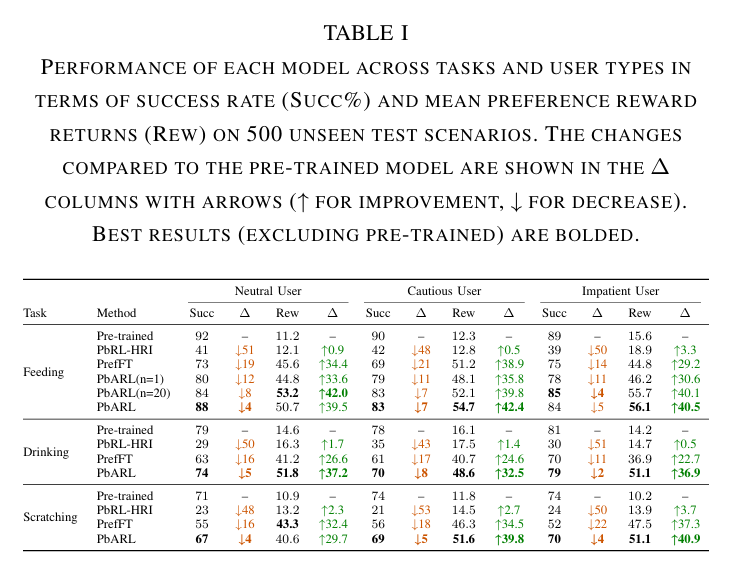
\includegraphics[width=\linewidth,height=0.72\textheight,keepaspectratio]{uploads/Screenshot 2026-06-08 140015.png}
\end{column}
\end{columns}
\end{frame}

% -------------------- Slide 19 --------------------
\begin{frame}{Real Robot Experiments}
\footnotesize
\begin{columns}[T,onlytextwidth]
\begin{column}{0.45\textwidth}
\textbf{Setup:}
\begin{itemize}\footnotesize
    \item Kinova Jaco arm
    \item RealSense camera
    \item Mouth tracking system
    \item Safety stop mechanism
\end{itemize}

\textbf{Results:}
\begin{itemize}\footnotesize
    \item Higher user satisfaction
    \item Better personalization
    \item Stable behavior
\end{itemize}
\end{column}
\begin{column}{0.52\textwidth}
\centering
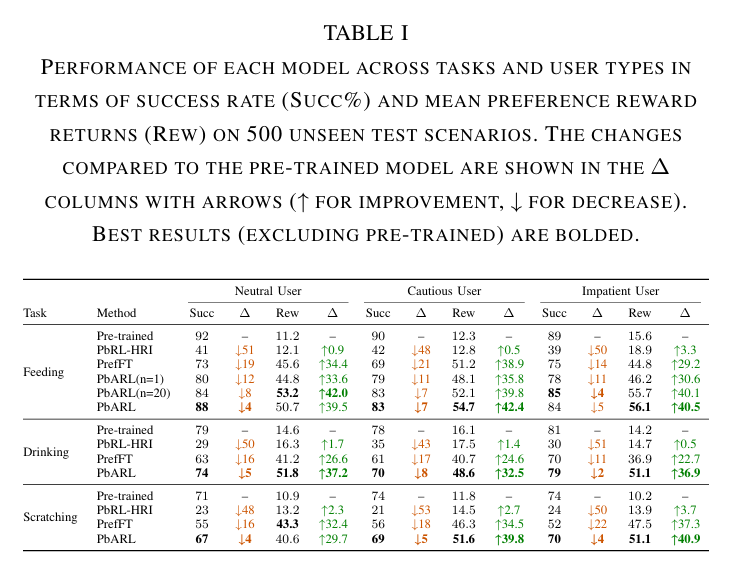
\includegraphics[width=\linewidth,height=0.72\textheight,keepaspectratio]{uploads/Screenshot 2026-06-08 140015.png}
\end{column}
\end{columns}
\end{frame}

% -------------------- Slide 20 --------------------
\begin{frame}{Conclusion}
\footnotesize
\textbf{Key idea}

\begin{itemize}\footnotesize
    \item Do not change the robot
    \item Change action representation
\end{itemize}

\vspace{0.5em}
\textbf{Final takeaway:} Personalization without forgetting
\end{frame}

% ============================================================
\section{Paper 4: Tozadore et al.\ (2018)}
% ============================================================

% \begin{frame}{Problem and setup}
%   \footnotesize \emph{Towards adaptation and personalization in task based on Human-Robot Interaction}, LARS/SBR 2018. \refnum{Tozadore2018}
%   \vspace{0.4em}
%   \begin{columns}[T]
%     \begin{column}{0.52\textwidth}
%       \textbf{The problem}
%       \begin{itemize}\footnotesize
%         \item Social robots lose novelty, so motivation and attention drop.
%         \item Hypothesis: personalized conversation and content adaptation hold interest longer.
%       \end{itemize}
%       \textbf{Contribution}
%       \begin{itemize}\footnotesize
%         \item A dynamic user-adaptation system (vs.\ the usual static user models).
%         \item Reads body and verbal signals to adjust behavior; stores user info to personalize dialogue.
%       \end{itemize}
%     \end{column}
%     \begin{column}{0.46\textwidth}
%       \textbf{Setup (worth noting)}
%       \begin{itemize}\footnotesize
%         \item Robot: NAO, with 10 real participants.
%         \item Task: a storytelling activity.
%         \item Decision-making is rule-based, not RL --- ML is used only for perception.
%         \item This is the ``before-RL'' approach: hand-tuned weighted rules.
%       \end{itemize}
%     \end{column}
%   \end{columns}
% \end{frame}

% \begin{frame}{Methodology}
%   \begin{columns}[T]
%     \begin{column}{0.5\textwidth}
%       \textbf{Decision logic (rule-based)}
%       \footnotesize
%       Three indicator groups $\rightarrow$ parameters:
%       \begin{itemize}\footnotesize
%         \item Attention $\alpha$: face gaze, posture
%         \item Communication $\beta$: words, emotion
%         \item Task $\gamma$: success rate, answer time
%       \end{itemize}
%       \[ F_{\text{Adp}}(t)=w_\alpha\alpha + w_\beta\beta + w_\gamma\gamma \]
%       {\scriptsize $\ge 0.66 \to {+}1$, $\le 0.33 \to {-}1$, else $0$; behavior $\Psi\!\in\!\{1..5\}$ (info $\leftrightarrow$ gesture), starts at 3. Weights set by hand: $w_\gamma{=}0.6$, $w_\alpha{=}w_\beta{=}0.2$.}
%     \end{column}
%     \begin{column}{0.5\textwidth}
%       \textbf{Perception (the ML part)}
%       \begin{itemize}\footnotesize
%         \item Face / gaze: Haar cascade.
%         \item Emotion: MobileNet, Ekman 6+neutral; trained on FER+, RAF, QIDER.
%         \item Answer check: Levenshtein edit distance.
%       \end{itemize}
%       \textbf{User model}
%       \begin{itemize}\footnotesize
%         \item Stores name, age, 8 preferences (sport, food, band\ldots).
%         \item Pulls definitions from Wikipedia to chat about them; gives NAO a ``personal life'' for rapport.
%       \end{itemize}
%     \end{column}
%   \end{columns}
% \end{frame}

% \begin{frame}{Results}
%   \begin{columns}[c,onlytextwidth]
%     \begin{column}{0.56\textwidth}
%       \centering
%       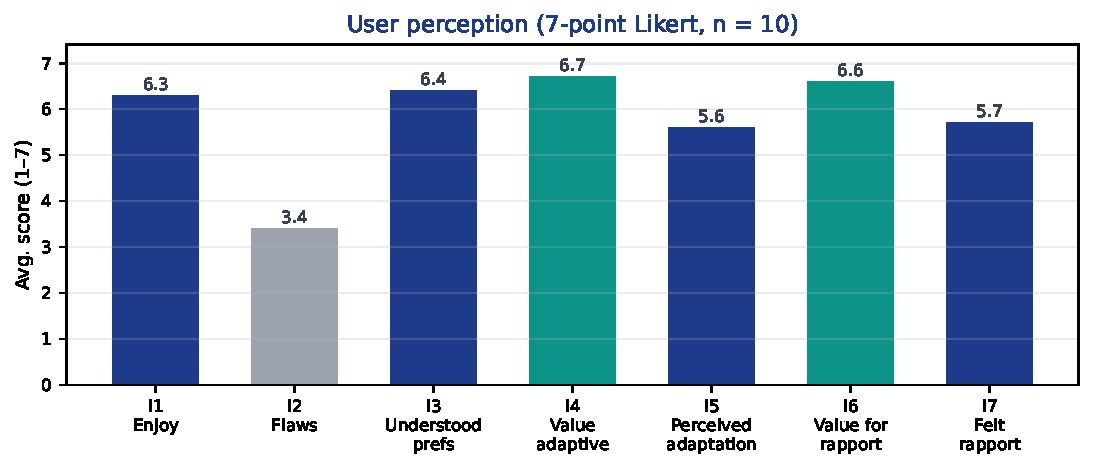
\includegraphics[width=\linewidth]{tozadore_likert.pdf}
%     \end{column}
%     \begin{column}{0.42\textwidth}
%       \footnotesize
%       \textbf{Protocol}: 10 users ($\bar{x}_{\text{age}}{=}24.4$), $\sim$12 min each; NAO greets, learns 3 preferences, tells 3 stories, quizzes, chats.
%       \medskip
%       \textbf{Reading it}
%       \begin{itemize}\footnotesize
%         \item Users value adaptation (I4 6.7, I6 6.6) more than they perceived it (I5 5.6, I7 5.7).
%         \item Enjoyment high (I1 6.3); flaws low (I2 3.4).
%         \item Task-success gain was not significant ($p{=}0.12$).
%       \end{itemize}
%     \end{column}
%   \end{columns}
%   \vspace{0.2em}
%   {\scriptsize Likert chart redrawn from Tozadore et al.\ (2018), Fig.\ 4 (real published values). \refnum{Tozadore2018}}
% \end{frame}

% \begin{frame}{Critique and relevance}
%   \begin{columns}[T]
%     \begin{column}{0.5\textwidth}
%       \textbf{Strengths}
%       \begin{itemize}\footnotesize
%         \item Real users on NAO (not simulation), with a usable evaluation template.
%         \item Genuine personalization (preferences, rapport) and honest negative findings.
%       \end{itemize}
%       \textbf{Gaps}
%       \begin{itemize}\footnotesize
%         \item Hand-tuned weights --- no learning; brittle to re-tune.
%         \item Perception fragile: edit distance misses paraphrases; Ekman emotions misread concentration.
%         \item Small sample (10), short single session; effect not significant.
%       \end{itemize}
%     \end{column}
%     \begin{column}{0.5\textwidth}
%       \textbf{Relevance to us}
%       \begin{itemize}\footnotesize
%         \item Completes the arc: personalization on NAO works with hand-coded rules --- so let RL learn the policy instead.
%         \item Their Likert items are a ready evaluation template for a user study.
%         \item Their failure modes tell us what to design around.
%       \end{itemize}
%     \end{column}
%   \end{columns}
% \end{frame}

%------------------------------------------------

\begin{frame}{Problem and Setup}
\footnotesize \emph{Towards Adaptation and Personalization in Task-Based Human-Robot Interaction}, LARS/SBR 2018. \refnum{Tozadore2018}

\vspace{0.4em}

\begin{columns}[T]

\begin{column}{0.52\textwidth}
\textbf{The problem}
\begin{itemize}\footnotesize
    \item Social robots lose novelty over time.
    \item Users become less engaged and less motivated.
    \item Question: can personalization sustain engagement?
\end{itemize}

\textbf{Contribution}
\begin{itemize}\footnotesize
    \item Dynamic adaptation system for HRI.
    \item Continuously adjusts robot behavior using user signals.
    \item Builds user-specific interaction history.
\end{itemize}
\end{column}

\begin{column}{0.46\textwidth}
\textbf{Setup (worth noting)}
\begin{itemize}\footnotesize
    \item Robot: NAO humanoid robot.
    \item Task: storytelling interaction.
    \item 10 participants (12 min sessions).
    \item Rule-based decision system (no RL).
\end{itemize}
\end{column}

\end{columns}
\end{frame}

%------------------------------------------------

\begin{frame}{Motivation}
\footnotesize

\begin{columns}[T]

\begin{column}{0.5\textwidth}
\textbf{Why adaptation matters}
\begin{itemize}\footnotesize
    \item Users differ in preferences and engagement levels.
    \item One fixed robot behavior is insufficient.
    \item Engagement decreases without personalization.
\end{itemize}

\textbf{Analogy}
\begin{itemize}\footnotesize
    \item Netflix → personalized recommendations
    \item YouTube → adaptive content feed
    \item Learning systems → adaptive difficulty
\end{itemize}
\end{column}

\begin{column}{0.5\textwidth}
\textbf{Goal in robotics}
\begin{itemize}\footnotesize
    \item Detect user state in real time.
    \item Adapt interaction style dynamically.
    \item Maintain long-term engagement.
\end{itemize}
\end{column}

\end{columns}
\end{frame}

%------------------------------------------------

\begin{frame}{System Overview}
\footnotesize
\begin{columns}[T,onlytextwidth]
\begin{column}{0.42\textwidth}
\textbf{Main idea}

\begin{itemize}\footnotesize
    \item The robot continuously monitors:
    \begin{itemize}\footnotesize
        \item Attention
        \item Communication
        \item Learning performance
    \end{itemize}
    \item Then adapts behavior accordingly.
\end{itemize}

\vspace{0.5em}

\textbf{Feedback loop}
\begin{itemize}\footnotesize
    \item Observe user $\rightarrow$ Estimate state $\rightarrow$ Compute score $\rightarrow$ Adapt behavior
\end{itemize}
\end{column}
\begin{column}{0.55\textwidth}
\centering
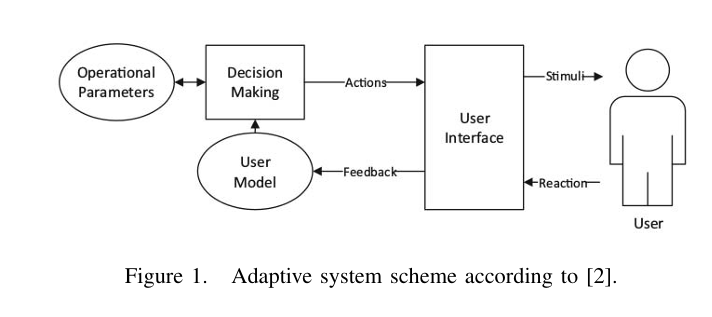
\includegraphics[width=\linewidth,height=0.72\textheight,keepaspectratio]{prism-uploads/Screenshot 2026-06-08 155900.png}
\end{column}
\end{columns}
\end{frame}

%------------------------------------------------

\begin{frame}{User State Estimation}
\footnotesize

\begin{columns}[T]

\begin{column}{0.33\textwidth}
\textbf{Attention ($\alpha$)}
\begin{itemize}\footnotesize
    \item Face gaze tracking
    \item Posture analysis
    \item Absence from camera
\end{itemize}
\end{column}

\begin{column}{0.33\textwidth}
\textbf{Communication ($\beta$)}
\begin{itemize}\footnotesize
    \item Number of words
    \item Emotion recognition
    \item Facial expression classification
\end{itemize}
\end{column}

\begin{column}{0.33\textwidth}
\textbf{Learning ($\gamma$)}
\begin{itemize}\footnotesize
    \item Answer correctness
    \item Response time
    \item Task success rate
\end{itemize}
\end{column}

\end{columns}

\vspace{0.6em}
\centering
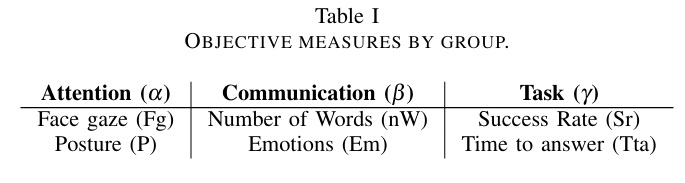
\includegraphics[width=0.9\linewidth,height=0.28\textheight,keepaspectratio]{prism-uploads/Screenshot 2026-06-08 164442.png}

\end{frame}

%------------------------------------------------

\begin{frame}{Emotion Recognition Module}
\footnotesize

\begin{columns}[T]

\begin{column}{0.55\textwidth}
\textbf{Model}
\begin{itemize}\footnotesize
    \item MobileNet (lightweight CNN)
    \item Trained on FER+, RAF, QIDER datasets
    \item Real-time emotion classification
\end{itemize}

\textbf{Emotion classes}
\begin{itemize}\footnotesize
    \item Happy, Sad, Angry, Fear
    \item Surprise, Disgust, Neutral
\end{itemize}
\end{column}

\begin{column}{0.45\textwidth}
\textbf{Why MobileNet?}
\begin{itemize}\footnotesize
    \item Fast inference
    \item Low computational cost
    \item Suitable for robotics hardware
\end{itemize}
\end{column}

\end{columns}

\end{frame}

%------------------------------------------------

\begin{frame}{Face Gaze and Answer Evaluation}
\footnotesize

\begin{columns}[T]

\begin{column}{0.5\textwidth}
\textbf{Face gaze tracking}
\begin{itemize}\footnotesize
    \item Haar cascade face detection
    \item Measures time away from robot
    \item Long absence → reduced attention
\end{itemize}
\end{column}

\begin{column}{0.5\textwidth}
\textbf{Answer evaluation}
\begin{itemize}\footnotesize
    \item Levenshtein distance
    \item Measures text similarity
    \item Small distance → correct answer
\end{itemize}
\end{column}

\end{columns}

\end{frame}

%------------------------------------------------

\begin{frame}{Adaptation Function}
\footnotesize

\textbf{Core equation}

\[
F_{Adp}(t) = w_{\alpha}\alpha(t) + w_{\beta}\beta(t) + w_{\gamma}\gamma(t)
\]

\vspace{0.5em}

\begin{itemize}\footnotesize
    \item $\alpha$: attention
    \item $\beta$: communication
    \item $\gamma$: learning performance
    \item Weights: 0.2, 0.2, 0.6
\end{itemize}

\vspace{0.5em}

\textbf{Decision rule}
\begin{itemize}\footnotesize
    \item $\geq 0.66$ → increase interaction
    \item $\leq 0.33$ → decrease interaction
    \item otherwise → maintain behavior
\end{itemize}

\end{frame}

%------------------------------------------------

\begin{frame}{Robot Behavior States}
\footnotesize

\begin{itemize}\footnotesize
    \item State 1: minimal interaction, low gestures
    \item State 2: slightly interactive
    \item State 3: neutral behavior
    \item State 4: more expressive
    \item State 5: highly social and engaging
\end{itemize}

\vspace{0.5em}

\textbf{Goal:} dynamically shift between states based on user engagement

\end{frame}

%------------------------------------------------

\begin{frame}{Experiment Setup}
\footnotesize

\begin{columns}[T]

\begin{column}{0.5\textwidth}
\textbf{Setup}
\begin{itemize}\footnotesize
    \item NAO humanoid robot
    \item 10 participants (students)
    \item 12-minute interactions
\end{itemize}

\textbf{Task}
\begin{itemize}\footnotesize
    \item Storytelling activity
    \item Questions after each story
\end{itemize}
\end{column}

\begin{column}{0.5\textwidth}
\textbf{Collected signals}
\begin{itemize}\footnotesize
    \item Attention
    \item Communication
    \item Learning performance
\end{itemize}
\end{column}

\end{columns}

\end{frame}

%------------------------------------------------

\begin{frame}{Results and Findings}
\footnotesize

\begin{itemize}\footnotesize
    \item Users reported high enjoyment.
    \item Perceived personalization improved engagement.
    \item Adaptive behavior improved interaction quality.
\end{itemize}

\vspace{0.5em}

\textbf{Key insight:}
Personalization increases perceived social presence of the robot.

\end{frame}

%------------------------------------------------

\begin{frame}{Limitations and Future Work}
\footnotesize

\begin{columns}[T]

\begin{column}{0.5\textwidth}
\textbf{Limitations}
\begin{itemize}\footnotesize
    \item Small sample size (10 users)
    \item Short interaction time
    \item Emotion confusion (concentration vs sadness)
    \item Weak semantic understanding
\end{itemize}
\end{column}

\begin{column}{0.5\textwidth}
\textbf{Future work}
\begin{itemize}\footnotesize
    \item Better emotion recognition models
    \item Long-term studies
    \item Improved language understanding
    \item Automatic user identification
\end{itemize}
\end{column}

\end{columns}

\end{frame}

%------------------------------------------------

\begin{frame}{Takeaway}
\footnotesize

\textbf{Core message}

\begin{itemize}\footnotesize
    \item Observe user behavior
    \item Estimate engagement (attention, communication, learning)
    \item Adapt robot behavior dynamically
    \item Personalize interaction using user memory
\end{itemize}

\vspace{0.5em}

\textbf{Final idea:}
Adaptive + personalized robots can sustain human engagement over time.

\end{frame}

% \begin{frame}{Problem and setup}
%   \footnotesize \emph{Personalization in HRI through Preference-based Action Representation Learning} (PbARL), arXiv 2025. \refnum{Wang2025}
%   \vspace{0.4em}
%   \begin{columns}[T]
%     \begin{column}{0.52\textwidth}
%       \textbf{The shift: learn the reward}
%       \begin{itemize}\footnotesize
%         \item The other papers hand-design the reward (comfort, engagement, weights) --- hard and brittle.
%         \item Preference-based RL: show the person two behaviors, ask which they prefer, and learn the reward from those comparisons.
%       \end{itemize}
%       \textbf{The problem they fix}
%       \begin{itemize}\footnotesize
%         \item Existing preference-based RL trains a policy from scratch per user, wasting feedback on the basic task.
%       \end{itemize}
%     \end{column}
%     \begin{column}{0.46\textwidth}
%       \textbf{Setup (worth noting)}
%       \begin{itemize}\footnotesize
%         \item Robot: Kinova Jaco assistive arm (not a humanoid).
%         \item Assistive Gym simulation + a real user study (N=8).
%         \item Frontier and heavy: deep RL, a variational autoencoder, 3 GPUs --- the opposite end from a laptop tabular approach.
%       \end{itemize}
%     \end{column}
%   \end{columns}
% \end{frame}

% \begin{frame}{Methodology}
%   \begin{columns}[T]
%     \begin{column}{0.5\textwidth}
%       \textbf{The core idea}
%       \begin{itemize}\footnotesize
%         \item Start from a frozen pre-trained policy that already knows the basic task.
%         \item Do not retrain it (that degrades the task). Instead, learn a latent action representation layered on top.
%         \item Train it to maximize the mutual information between the task domain and the preference-aligned domain.
%       \end{itemize}
%     \end{column}
%     \begin{column}{0.5\textwidth}
%       \textbf{Why it works}
%       \begin{itemize}\footnotesize
%         \item Naive fine-tuning optimizes only preference, which breaks the task.
%         \item PbARL balances both: one loss preserves the task, another aligns preferences.
%       \end{itemize}
%       \begin{block}{}
%         \scriptsize Far more complex than tabular Q-learning --- we cite it as the state of the art, not as something we replicate.
%       \end{block}
%     \end{column}
%   \end{columns}
% \end{frame}

% \begin{frame}{Results}
%   \begin{columns}[c,onlytextwidth]
%     \begin{column}{0.54\textwidth}
%       \centering
%       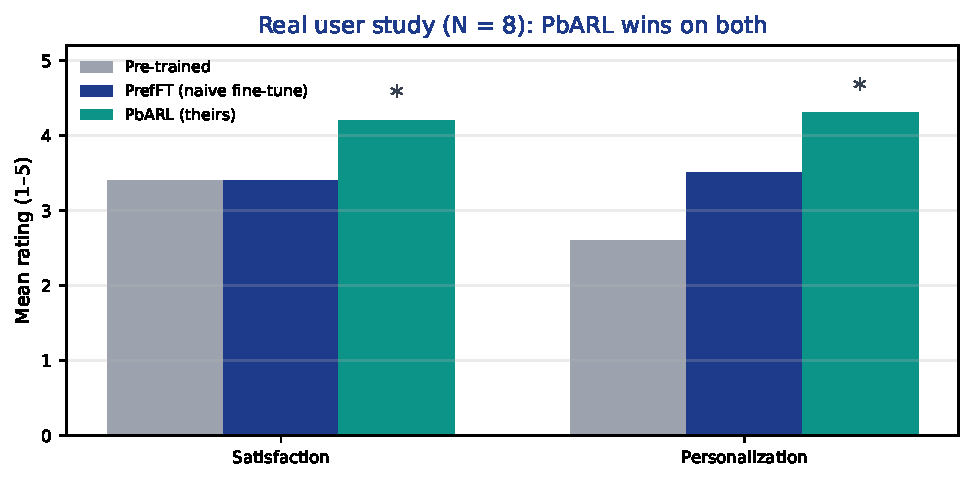
\includegraphics[width=\linewidth]{wang_userstudy.pdf}
%     \end{column}
%     \begin{column}{0.44\textwidth}
%       \footnotesize
%       \textbf{Benchmark (Assistive Gym)}
%       \begin{itemize}\footnotesize
%         \item PbARL keeps task success (only $\downarrow$4--7) and boosts preference reward ($\sim$+40).
%         \item Naive fine-tuning drops success $\downarrow$11--22; from-scratch RL collapses ($\downarrow$48--53).
%       \end{itemize}
%       \textbf{Real study (N=8)}: PbARL best on both satisfaction and personalization ($p<.01$).
%     \end{column}
%   \end{columns}
%   \vspace{0.2em}
%   {\scriptsize User-study chart redrawn from Wang et al.\ (2025), Fig.\ 4; values approximate. \refnum{Wang2025}}
% \end{frame}

% \begin{frame}{Critique and relevance}
%   \begin{columns}[T]
%     \begin{column}{0.5\textwidth}
%       \textbf{Strengths}
%       \begin{itemize}\footnotesize
%         \item Learns the reward from preferences --- no hand-design.
%         \item Personalizes without degrading the task; real IRB-approved user study.
%       \end{itemize}
%       \textbf{Gaps}
%       \begin{itemize}\footnotesize
%         \item Assistive arm, not a humanoid; heavy compute (3 GPUs).
%         \item Complex pipeline; preferences treated as fixed; N=8.
%       \end{itemize}
%     \end{column}
%     \begin{column}{0.5\textwidth}
%       \textbf{Relevance to us}
%       \begin{itemize}\footnotesize
%         \item Defines the frontier: where reward design is heading.
%         \item Justifies our scope by contrast: we start simple, interpretable, and laptop-trainable.
%         \item A clear future direction: replace a hand-set reward with learned preferences.
%       \end{itemize}
%     \end{column}
%   \end{columns}
% \end{frame}

% ============================================================
\section{Synthesis}
% ============================================================

\begin{frame}{Gaps across the four papers}
  \footnotesize
  \begin{itemize}
    \item \textbf{Reward design:} hand-designed (Tozadore, Gonzalez, Zedda) is brittle; learned preferences (Wang) are powerful but heavy. \emph{We start with a simple explicit reward; learned preferences are future work.}
    \item \textbf{Simulation vs.\ real:} simulation dominates training (Gonzalez, Wang's benchmark); real studies are still small (Tozadore $n{=}10$, Wang $N{=}8$, Zedda $N{=}28$). \emph{We go simulation-first, then a small real study.}
    \item \textbf{Platform:} industrial arms (Gonzalez, Wang) vs.\ humanoids (Zedda's Pepper, Tozadore's NAO). \emph{We target a humanoid.}
    \item \textbf{Method complexity:} deep RL on GPUs (Gonzalez, Wang) vs.\ lightweight tabular (Zedda). \emph{We stay interpretable and feasible.}
    \item \textbf{Evaluation:} subjective surveys dominate. \emph{We combine objective sensor metrics with subjective scales.}
  \end{itemize}
  \begin{block}{}
    \footnotesize Our project sits where these gaps overlap: a humanoid, a simple interpretable RL method, a live reward signal, and an evaluation that triangulates both kinds of metric.
  \end{block}
\end{frame}

% ============================================================
\section{Platform and feasibility}
% ============================================================

\begin{frame}{Platform and feasibility}
  We have kept our setup robot-agnostic, because a few practical questions are still open and the answers shape the project:
  \begin{itemize}
    \item Is \textbf{NAO} still the platform you would like us to use in 2026, or is there a newer or preferred one?
    \item Will a physical NAO realistically be \textbf{available before the end of the semester}?
    \item If not, should we focus \textbf{entirely on simulation}?
    \item And should simulation stay \textbf{NAO-compatible}, or are entirely different directions acceptable?
  \end{itemize}
  \vspace{0.3em}
  \begin{block}{}
    \footnotesize Our initial setup does not assume NAO specifically, so we can adapt to whichever answer you give.
  \end{block}
\end{frame}

\begin{frame}{What NAO offers, if it is the platform}
  \begin{columns}[T]
    \begin{column}{0.5\textwidth}
      \textbf{Hardware} \refnum{Aldebaran}
      \begin{itemize}\footnotesize
        \item 58\,cm, $\sim$5.6\,kg, 25 degrees of freedom
        \item Dual cameras; 4 microphones
        \item Sonar distance sensors ($\sim$25--255\,cm)
        \item Tactile sensors (head + hands); foot force sensors; IMU
        \item Battery $\sim$45--90\,min; limited onboard compute
      \end{itemize}
    \end{column}
    \begin{column}{0.5\textwidth}
      \textbf{Software (NAOqi SDK)}
      \begin{itemize}\footnotesize
        \item \texttt{ALMotion} --- joints, posture, walking
        \item \texttt{ALMemory} / \texttt{ALSensors} --- sensor access
        \item \texttt{ALSonar} --- distance; \texttt{ALTextToSpeech} --- speech
        \item Choregraphe IDE (with a virtual NAO)
        \item Python / C++ SDKs; ROS support
      \end{itemize}
    \end{column}
  \end{columns}
  \vspace{0.4em}
  {\footnotesize Sonar and tactile sensors give a clean, real-time signal for a comfort- or engagement-based reward --- which is what makes a humanoid like NAO a natural fit \emph{if} it is available.}
\end{frame}

% ============================================================
\section{Project directions}
% ============================================================

\begin{frame}{Candidate directions}
  \footnotesize We are not committing yet --- these share one RL loop; only the state, actions, and reward differ. We would like the discussion to help pick one (or suggest another).
  \begin{table}
    \begin{tabular}{@{}>{\raggedright\arraybackslash}p{2.4cm}>{\raggedright\arraybackslash}p{3.1cm}>{\raggedright\arraybackslash}p{3.0cm}>{\raggedright\arraybackslash}p{2.6cm}@{}}
      \toprule
      \textbf{Direction} & \textbf{Adaptive behavior} & \textbf{Reward signal} & \textbf{Baseline} \\
      \midrule
      Greeting / social distance & Approach distance + greeting intensity & Tactile ``approve'' + sonar distance & Fixed scripted greeting \\
      \addlinespace
      Tutoring / pace & Speech rate, pauses, difficulty & Answer correctness + engagement & Fixed-pace tutor \\
      \addlinespace
      Engagement & Pick from a behavior repertoire & Change in gaze + proximity & Random / fixed rotation \\
      \bottomrule
    \end{tabular}
  \end{table}
  \vspace{0.3em}
  {\footnotesize Illustrated here on a NAO-like humanoid, but the same structure ports to a simulator or another platform.}
\end{frame}

\begin{frame}{Initial technical setup}
  \footnotesize
  We have started building a small, robot-agnostic RL loop. We expect most of it to be reusable across whichever direction we choose --- it is early groundwork, not a finished system.
  \vspace{0.3em}
  \begin{columns}[c,onlytextwidth]
    \begin{column}{0.46\textwidth}
      \centering
      \resizebox{\linewidth}{!}{%
      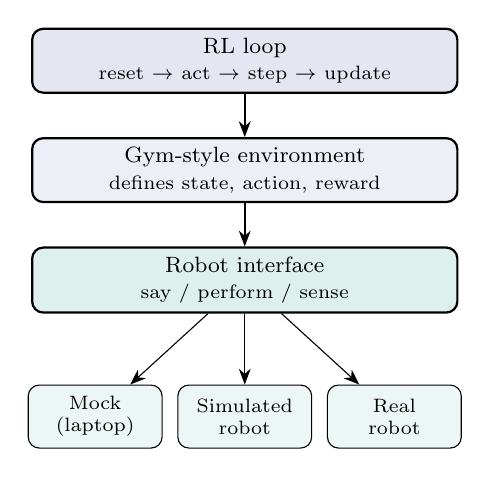
\begin{tikzpicture}[
        node distance=0.55cm,
        layer/.style={draw, rounded corners, minimum width=5.4cm, minimum height=0.8cm, align=center, thick, font=\footnotesize},
        impl/.style={draw, rounded corners, minimum width=1.7cm, minimum height=0.8cm, align=center, font=\scriptsize}]
        \node[layer, fill=giublue!12] (loop) {RL loop \\ {\scriptsize reset $\to$ act $\to$ step $\to$ update}};
        \node[layer, fill=giublue!8, below=of loop] (env) {Gym-style environment \\ {\scriptsize defines state, action, reward}};
        \node[layer, fill=giuaccent!14, below=of env] (iface) {Robot interface \\ {\scriptsize say / perform / sense}};
        \node[impl, fill=giuaccent!8, below=0.9cm of iface, xshift=-1.9cm] (mock) {Mock \\ (laptop)};
        \node[impl, fill=giuaccent!8, below=0.9cm of iface] (sim) {Simulated \\ robot};
        \node[impl, fill=giuaccent!8, below=0.9cm of iface, xshift=1.9cm] (real) {Real \\ robot};
        \draw[-{Stealth[length=2mm]}, thick] (loop)--(env);
        \draw[-{Stealth[length=2mm]}, thick] (env)--(iface);
        \draw[-{Stealth[length=2mm]}] (iface)--(mock);
        \draw[-{Stealth[length=2mm]}] (iface)--(sim);
        \draw[-{Stealth[length=2mm]}] (iface)--(real);
      \end{tikzpicture}%
      }
    \end{column}
    \begin{column}{0.50\textwidth}
      \begin{itemize}\footnotesize
        \item The learning code talks to an abstract \emph{interface}, not a specific robot.
        \item An early prototype runs in simulation against a mock that includes a simulated person.
        \item Sensor noise is injected to make the policy more robust.
        \item Moving to a simulated or real robot mainly means providing a new implementation of the interface.
      \end{itemize}
    \end{column}
  \end{columns}
\end{frame}

\begin{frame}[fragile]{A robot-agnostic interface (early prototype)}
  \scriptsize
  The interface is the seam that lets the same learning code run against a mock, a simulator, or a real robot. The mock includes a simulated person, so the loop runs with no hardware.
\begin{semiverbatim}\scriptsize
class RobotInterface(ABC):           \textcolor{gray}{# shared by mock / sim / real}
    def perform(self, action): ...   \textcolor{gray}{# 'closer','back','intensity_up'...}
    def sense(self) -> Signals: ...  \textcolor{gray}{# {distance, touch, present}}

class MockRobot(RobotInterface):     \textcolor{gray}{# laptop + simulated person}
    def sense(self):
        return Signals(distance=self._d + noise,
                       touch=self._person_approves(),
                       present=self._present)
\end{semiverbatim}
  \vspace{-0.2em}
  Early result: in simulation it learns to approach to a comfortable distance and hold, rather than crowd the person --- a clear improvement over a fixed script. Hosted on GitHub.
\end{frame}

\begin{frame}{An illustrative MDP (greeting)}
  {\footnotesize Not our chosen experiment --- an illustration of how any direction becomes a concrete MDP. This is the one we prototyped to check the architecture.}
  \vspace{0.3em}
  \begin{columns}[T]
    \begin{column}{0.5\textwidth}
      \textbf{State} (discretized)
      \begin{itemize}\footnotesize
        \item Distance bin: intimate / personal / social
        \item Current greeting intensity
      \end{itemize}
      \textbf{Action}
      \begin{itemize}\footnotesize
        \item move closer / move back
        \item increase / decrease intensity / hold
      \end{itemize}
    \end{column}
    \begin{column}{0.5\textwidth}
      \textbf{Reward}
      \begin{itemize}\footnotesize
        \item $+$ head touch, sustained gaze, user stays
        \item $-$ user steps back, no touch, leaves
      \end{itemize}
      \textbf{Algorithm}
      \begin{itemize}\footnotesize
        \item Tabular Q-learning, $\varepsilon$-greedy
        \item Small discrete space, so it converges quickly
      \end{itemize}
    \end{column}
  \end{columns}
\end{frame}

\begin{frame}{Evaluation}
  \begin{columns}[T]
    \begin{column}{0.5\textwidth}
      \textbf{Study design}
      \begin{itemize}\footnotesize
        \item Within-subject: each participant meets the scripted and the learned robot (counterbalanced).
        \item Higher power; controls individual differences.
      \end{itemize}
      \textbf{Objective metrics}
      \begin{itemize}\footnotesize
        \item Convergence speed
        \item Final interaction distance, approach latency
        \item Engagement duration
      \end{itemize}
    \end{column}
    \begin{column}{0.5\textwidth}
      \textbf{Subjective metrics}
      \begin{itemize}\footnotesize
        \item Godspeed questionnaire (likeability, perceived safety, perceived intelligence)
        \item Comfort / trust survey
      \end{itemize}
      \textbf{The point}
      \begin{itemize}\footnotesize
        \item Triangulate: pair sensor metrics with subjective scales --- addressing the field's main critique.
      \end{itemize}
    \end{column}
  \end{columns}
\end{frame}

\begin{frame}{Implementation plan}
  \begin{enumerate}
    \item \textbf{Mock / Gym environment} (platform-agnostic): encode the state--action--reward MDP and verify the agent learns.
    \item \textbf{Simulated humanoid}: move to Choregraphe's virtual NAO or Webots --- or another simulator if preferred.
    \item \textbf{Real robot, if available}: fine-tune for a small number of trials; watch joint heat and battery.
    \item \textbf{If NAO is not available}: stay in simulation, or target a different platform --- the architecture does not assume NAO.
  \end{enumerate}
  \vspace{0.3em}
  \begin{block}{}
    \footnotesize Code is on GitHub, with a modular interface so the same RL loop runs against mock, simulator, or hardware.
  \end{block}
\end{frame}

% ============================================================
\section{Questions for the committee}
% ============================================================

\begin{frame}{Questions for the committee}
  \begin{columns}[T]
    \begin{column}{0.5\textwidth}
      \textbf{Platform (recap)}
      \begin{itemize}\footnotesize
        \item NAO or another platform? Available this semester?
        \item Simulation-only acceptable if not?
      \end{itemize}
      \textbf{Direction}
      \begin{itemize}\footnotesize
        \item Which direction should we pursue --- greeting, tutoring, engagement, or something you suggest?
      \end{itemize}
    \end{column}
    \begin{column}{0.5\textwidth}
      \textbf{Study logistics}
      \begin{itemize}\footnotesize
        \item May we recruit fellow students as participants?
        \item What ethics / consent process is required?
      \end{itemize}
      \textbf{Compute}
      \begin{itemize}\footnotesize
        \item Tabular Q-learning runs on a laptop --- no GPU needed.
        \item Only a deep-RL extension would need compute --- is any available?
      \end{itemize}
    \end{column}
  \end{columns}
\end{frame}

\begin{frame}[allowframebreaks]{References}
  \footnotesize
  \begin{thebibliography}{99}
    \setbeamertemplate{bibliography item}[text]

    \bibitem{Gonzalez2024} A.\ Gonzalez-Santocildes, J.-I.\ Vazquez, A.\ Eguiluz,
      ``Adaptive Robot Behavior Based on Human Comfort Using Reinforcement Learning,''
      \emph{IEEE Access}, vol.\ 12, pp.\ 122289--122299, 2024.
      DOI: 10.1109/ACCESS.2024.3451663.

    \bibitem{Zedda2023} E.\ Zedda, M.\ Manca, F.\ Patern\`o, C.\ Santoro,
      ``An Adaptive Behaviour-Based Strategy for SARs interacting with Older Adults with MCI during a Serious Game Scenario,''
      \emph{SARs Workshop (TMI), CHI 2023}, Hamburg, 2023. arXiv:2305.01492.
      (Extended: \emph{Behaviour \& Information Technology}, 2025.)

    \bibitem{Zedda2025} E.\ Zedda, M.\ Manca, F.\ Patern\`o, C.\ Santoro,
      ``Adaptive Humanoid Robot Behaviour in a Serious Game Scenario through Reinforcement Learning,''
      \emph{Behaviour \& Information Technology}, 2025.

    \bibitem{Tozadore2018} D.\ C.\ Tozadore et al.,
      ``Towards Adaptation and Personalization in Task Based on Human-Robot Interaction,''
      \emph{LARS/SBR/WRE}, 2018, pp.\ 383--389.
      DOI: 10.1109/LARS/SBR/WRE.2018.00075.

    \bibitem{Wang2025} R.\ Wang, D.\ Zhao, D.\ Suh, Z.\ Yuan, G.\ Chen, B.-C.\ Min,
      ``Personalization in Human-Robot Interaction through Preference-based Action Representation Learning,''
      arXiv:2409.13822, 2025.

    \bibitem{Mitsunaga2005} N.\ Mitsunaga, C.\ Smith, T.\ Kanda, H.\ Ishiguro, N.\ Hagita,
      ``Robot behavior adaptation for HRI based on policy gradient reinforcement learning,''
      \emph{IEEE/RSJ IROS}, 2005, pp.\ 218--225. DOI: 10.1109/IROS.2005.1545206.
      (Journal: \emph{IEEE T-RO} 24(4):911--916, 2008.)

    \bibitem{Pollmann2023} K.\ Pollmann, W.\ Loh, N.\ Fronemann, D.\ Ziegler,
      ``Entertainment vs.\ manipulation: Personalized human-robot interaction,''
      \emph{Technological Forecasting and Social Change}, vol.\ 189, art.\ 122376, 2023.
      DOI: 10.1016/j.techfore.2023.122376.

    \bibitem{Irfan2019} B.\ Irfan et al.,
      ``Personalization in Long-Term Human-Robot Interaction,''
      \emph{14th ACM/IEEE Int. Conf. on HRI}, 2019, pp.\ 685--686.
      DOI: 10.1109/HRI.2019.8673076.

    \bibitem{Irfan2021} B.\ Irfan et al.,
      ``Lifelong Learning and Personalization in Long-Term HRI (LEAP-HRI),''
      \emph{Companion of the 2021 ACM/IEEE Int. Conf. on HRI}, 2021, pp.\ 724--727.
      DOI: 10.1145/3434074.3444881.

    \bibitem{Sutton2018} R.\ S.\ Sutton and A.\ G.\ Barto,
      \emph{Reinforcement Learning: An Introduction}, 2nd ed. MIT Press, 2018.

    \bibitem{Knox2009} W.\ B.\ Knox and P.\ Stone,
      ``Interactively Shaping Agents via Human Reinforcement: The TAMER Framework,''
      \emph{K-CAP}, 2009. DOI: 10.1145/1597735.1597738.

    \bibitem{Argall2009} B.\ Argall, S.\ Chernova, M.\ Veloso, B.\ Browning,
      ``A survey of robot learning from demonstration,''
      \emph{Robotics and Autonomous Systems}, 57(5):469--483, 2009.
      DOI: 10.1016/j.robot.2008.10.024.

    \bibitem{Aldebaran} Aldebaran (SoftBank Robotics),
      \emph{NAO6 Documentation \& User Guide}. doc.aldebaran.com.

  \end{thebibliography}
\end{frame}

\begin{frame}[standout]
  A closing thought
  \vspace{1.2em}

  {\large If the robot's reward is our approval,\\
  it learns what pleases us --- not necessarily what is good for us.}
  \vspace{1.2em}

  {\normalsize Designing for that gap --- comfort versus manipulation --- \\ may be the real research question behind adaptive robots.}
\end{frame}

\begin{frame}[standout]
  Thank you\\[0.4em]
  {\normalsize Nour Gaser \& Eman Saleh}
\end{frame}

% ============================================================
\appendix
% ============================================================

\begin{frame}{Appendix}
  \begin{center}
    \large Held in reserve for discussion and deeper questions.
  \end{center}
  \vspace{1em}
  \begin{enumerate}
    \item One Q-learning update, worked numerically
    \item Supervised vs.\ RL on the same task
    \item Why tabular Q-learning rather than deep RL
    \item Preference-based RL in brief
    \item Ethics: entertainment vs.\ manipulation
    \item The reality gap
  \end{enumerate}
\end{frame}

\begin{frame}{One Q-learning update, step by step}
  \footnotesize
  \textbf{Setup (greeting MDP).} $\alpha=0.5$, $\gamma=0.9$. Current estimate $Q(s_{\text{far}},\,\texttt{closer})=0.0$.
  \begin{enumerate}
    \item \textbf{State} $s_{\text{far}}$: person in the social distance bin.
    \item \textbf{Action} (via $\varepsilon$-greedy, exploiting): $a=\texttt{move closer}$.
    \item \textbf{Outcome:} person stays and gives a head touch, so reward $r=+1$.
    \item \textbf{Next state} $s'=s_{\text{personal}}$, where the current best value is $\max_{a'}Q(s',a')=0.4$.
  \end{enumerate}
  \vspace{0.3em}
  \begin{block}{Apply the update}
    \[
      Q(s_{\text{far}},\texttt{closer}) \leftarrow 0.0 + 0.5\big[\,1 + 0.9(0.4) - 0.0\,\big]
      = 0.5\,(1.36) = 0.68
    \]
  \end{block}
  \footnotesize The estimate rises from $0.0$ to $0.68$: ``moving closer from far was good here.'' Repeat over episodes and the table converges to a policy that approaches each person's comfortable distance. \refnum{Sutton2018}
\end{frame}

\begin{frame}{Supervised vs.\ RL on the same task}
  \footnotesize
  \textbf{Task: choose how close the robot stands when greeting a new person.}
  \begin{table}
    \begin{tabular}{@{}>{\raggedright\arraybackslash}p{2.1cm}>{\raggedright\arraybackslash}p{4.1cm}>{\raggedright\arraybackslash}p{4.7cm}@{}}
      \toprule
       & \textbf{Supervised learning} & \textbf{Reinforcement learning} \\
      \midrule
      Data needed & A large labeled set (person features $\to$ ``correct'' distance), gathered in advance & None up front --- learns from live reward (touch, sonar, dwell) \\
      \addlinespace
      When it learns & Offline, before deployment & Online, during interaction \\
      \addlinespace
      New person & Predicts from a fixed model; cannot adjust if wrong & Tries, observes feedback, corrects within the session \\
      \addlinespace
      Failure mode & Confidently wrong on anyone unlike the training data & Some early exploration cost before convergence \\
      \bottomrule
    \end{tabular}
  \end{table}
  \vspace{0.2em}
  The ``right'' social distance is personal and unknown in advance --- the setting where RL's online adaptation fits better than a pre-trained classifier.
\end{frame}

\begin{frame}{Why tabular Q-learning rather than deep RL}
  \begin{columns}[T]
    \begin{column}{0.5\textwidth}
      \textbf{Our setting}
      \begin{itemize}\footnotesize
        \item Small, discrete state and action space.
        \item A handful of distance bins and intensity levels.
      \end{itemize}
      \textbf{So tabular fits}
      \begin{itemize}\footnotesize
        \item One value per (state, action); updated with simple arithmetic.
        \item Runs on a laptop CPU; no GPU.
        \item Converges in seconds; fully interpretable (we can read the table).
      \end{itemize}
    \end{column}
    \begin{column}{0.5\textwidth}
      \textbf{When deep RL is needed}
      \begin{itemize}\footnotesize
        \item Large or continuous spaces (Gonzalez, Wang) --- hence SAC and GPUs.
        \item More expressive, but heavier, slower, and harder to interpret.
      \end{itemize}
      \begin{block}{}
        \scriptsize Starting tabular keeps the project feasible and explainable; deep RL is a clear future step if the state space grows.
      \end{block}
    \end{column}
  \end{columns}
\end{frame}

\begin{frame}{Preference-based RL in brief}
  \footnotesize
  A likely question after Paper 3: \emph{why not use preference-based RL?}
  \begin{itemize}
    \item \textbf{Idea:} instead of designing a reward, show the person two short behaviors and ask which they prefer. A model learns a reward from many such comparisons (Bradley--Terry).
    \item \textbf{Strength:} avoids hand-designing a reward --- the hardest part in the other papers.
    \item \textbf{Cost:} needs many comparisons and, in practice, deep RL and real compute (Wang: 3 GPUs).
  \end{itemize}
  \begin{block}{Our position}
    \footnotesize For a first project we use a simple explicit reward (touch, sonar, dwell) that is clean and interpretable. Replacing it with learned preferences is a natural extension once the basic loop works.
  \end{block}
\end{frame}

\begin{frame}{Ethics: entertainment vs.\ manipulation}
  \begin{columns}[T]
    \begin{column}{0.5\textwidth}
      \textbf{The risk \refnum{Pollmann2023}}
      \begin{itemize}\footnotesize
        \item Personalization that improves experience can also steer behavior against a person's autonomy.
        \item A robot optimizing ``engagement'' could learn manipulative tactics if the reward is naive.
        \item Vulnerable users (children, elderly) raise the stakes.
      \end{itemize}
    \end{column}
    \begin{column}{0.5\textwidth}
      \textbf{Our safeguards}
      \begin{itemize}\footnotesize
        \item Reward tied to comfort, not raw attention.
        \item Transparency: the person knows the robot is adapting.
        \item Informed consent and a right to stop, for every participant.
        \item Store only what the task needs.
      \end{itemize}
    \end{column}
  \end{columns}
\end{frame}

\begin{frame}{The reality gap}
  \footnotesize
  We prototype in simulation first, so we are clear about what that does and does not prove.
  \begin{columns}[T]
    \begin{column}{0.5\textwidth}
      \textbf{Why a gap exists}
      \begin{itemize}
        \item Real sonar and tactile readings are noisy; mocks are clean.
        \item Real people behave unpredictably; scripted ``users'' do not.
        \item Joint dynamics, latency, and timing differ on hardware.
      \end{itemize}
    \end{column}
    \begin{column}{0.5\textwidth}
      \textbf{How we reduce it}
      \begin{itemize}
        \item Inject noise into the mock sensors.
        \item Keep the state and action space small and discrete.
        \item Treat simulation as a convergence check; reserve real trials for fine-tuning.
        \item Report simulation and real results separately.
      \end{itemize}
    \end{column}
  \end{columns}
  \vspace{0.3em}
  \begin{block}{}
    \footnotesize Simulation shows the algorithm works; only the physical robot shows the interaction works.
  \end{block}
\end{frame}

\end{document}